\subsection{Current limitations}
\label{sec:current-limitations}
% Short intro
The bottom-up characterization method helps create higher-order models of circuit functions.
However, preliminary tests regarding this method are inconclusive.
Multiple sources of errors in the modeling method can be found to explain the differences observed.

\subsubsection{Impact of characterization output load and output modeling method}

% First source of error - load impedance
Previously, it was indicated that all characterization curves were extracted with a fixed output load.
In \ref{sec:application-test-vehicle}, the output load Zout was 1M\textOmega.
It is believed that this is the first major source of error.

% Compare 1Mohm with real case where blocks are connected together
In reality, each block (pre-regulator, bandgap, regulator) sees a load impedance on its output much different than 1M\textOmega.
For instance, the output of the pre-regulator is a supply.
As such, it can deliver about 20mA of current while maintaining 8V.
Thus, the minimum output load this block can sustain is 400\textOmega.
The bandgap, on the other hand, provides a reference voltage at 1V but does not deliver a lot of DC current.
More than 1uA is enough to make the output fall of a hundred millivolts.
In this case, the bandgap must see an output impedance of at least 1M\textOmega.

% What is done next
To evaluate the impact the pre-regulator is characterized again, this time with lower load values.
Variations on the input stresses and results are summarized in table \ref{tab:impact-load-on-cz}.

% Analyse the table - worst case
For the smallest 10V stress amplitude, the failure time is largely impacted by the output load.
This is especially true for long pulses.
The worst case is for the -10V 1us pulse.
The output goes below 0V for 1330 ns with 500\textOmega\ on the output, but with 1M\textOmega\, no failure is observed.

% Analyse the table - other cases
However, it is interesting to notice that for larger pulse amplitudes, the output load has a limited impact on the failure duration.
It seems that once the output is at fault, having 500\textOmega\ or 1M\textOmega\ connected to it doesn't change how long it remains at fault.
Fig. \ref{fig:impact-time-domain-load} provides a visual representation of the phenomenon, to try to explain why this result is obtained.
When the output is disturbed and its amplitude is near the failure criteria, the load value has a strong impact on the width of the failure.
Indeed, a large load value (1 M\textOmega) causes the output to be slightly above the failure criteria, thus no failure is recorded.
On the contrary, with a small load (500 \textOmega\) the output amplitude has changed a little bit and is now below the failure criteria.
It is interesting to notice that in the reference simulations, the width of the disturbance doesn't change much with the load.

%TODO: To do with more blocks

\begin{table}[!htbp]
\centering
\begin{tabular}{llll}
\toprule
load (\textOmega) & amplitude (V) & length (ns) & output disturbed (ns)   \\ \midrule
500               & -10        & 10         & 10n    \\
5k                &            &            & 1n    \\
50k               &            &            & None    \\
1M                &            &            & None    \\
\rowcolor[gray]{.95}
500               &            & 100        & 100n    \\ \rowcolor[gray]{.95}
5k                &            &            & 1n    \\ \rowcolor[gray]{.95}
50k               &            &            & None    \\ \rowcolor[gray]{.95}
1M                &            &            & None    \\

500               &            & 1000       & 1330n    \\
5k                &            &            & 1289n    \\
50k               &            &            & None    \\
1M                &            &            & None     \\
\rowcolor[gray]{.95}
500               & -30        & 10         & 20n    \\ \rowcolor[gray]{.95}
5k                &            &            & 10n    \\ \rowcolor[gray]{.95}
50k               &            &            & 10n    \\ \rowcolor[gray]{.95}
1M                &            &            & 10n    \\

500               &            & 100        &  506n   \\
5k                &            &            &  580n   \\
50k               &            &            &  594n   \\
1M                &            &            &  594n   \\
\rowcolor[gray]{.95}
500               &            & 1000       & 2087    \\ \rowcolor[gray]{.95}
5k                &            &            & 2194    \\ \rowcolor[gray]{.95}
50k               &            &            & 2206    \\ \rowcolor[gray]{.95}
1M                &            &            & 2206    \\

500               & -45        & 10         & 46n    \\
5k                &            &            & 10n    \\
50k               &            &            & 10n    \\
1M                &            &            & 10n    \\
\rowcolor[gray]{.95}
500               &            & 100        & 657n    \\ \rowcolor[gray]{.95}
5k                &            &            & 715n    \\ \rowcolor[gray]{.95}
50k               &            &            & 717n    \\ \rowcolor[gray]{.95}
1M                &            &            & 727n    \\

500               &            & 1000       & 2668n    \\
5k                &            &            & 2764n   \\
50k               &            &            & 2800n    \\
1M                &            &            & 2800n    \\

\bottomrule
\end{tabular}
\caption{Impact of the output load on characterization results}
\label{tab:impact-load-on-cz}
\end{table}

\begin{figure}[!htbp]
  \centering
  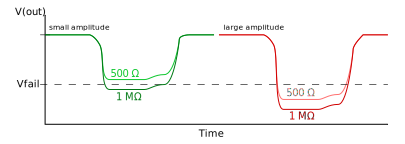
\includegraphics{src/4/figures/zout_impact_time_domain.pdf}
  \caption{Represented impact of output load impedance on the output waveform during a disturbance with a small amplitude (green) and a large amplitude (red)}
  \label{fig:impact-time-domain-load}
\end{figure}

% Conclusion, the main impact is not the characterization load, but the single failure criteria
In conclusion, the load value used during characterization does not seem to be the main source of error.
Rather, it is the consequence of using a single level as failure criteria, which eliminates a lot of information.
Basically, it oversimplifies the waveform of the output.
This is illustrated by figure. \ref{fig:impact-single-failure-criteria}.
Any disturbance under the failure criteria is modeled as no disturbance.
This is the case even if the disturbance is just below the failure criteria, without crossing it.
On the contrary, any disturbance beyond the failure criteria uses the failure level for modeling.
The max value of the output may be much larger than the failure criteria, however, it will still be modeled as a square pulse of amplitude Vfail.

\begin{figure}[!htbp]
  \centering
  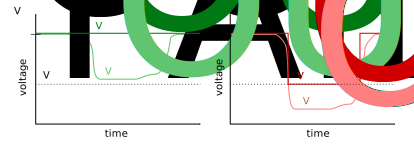
\includegraphics{src/4/figures/bad_output_modelling.pdf}
  \caption{Lack of accuracy caused by the use of a single failure criteria to model the output}
  \label{fig:impact-single-failure-criteria}
\end{figure}

% Talk about static impedances vs dynamic
%TODO: Not studied ?
% Talk about real vs imaginary impedances
%TODO: Not studied

\subsubsection{Other sources}

%TODO: Make section ? Speak about limitations with multiples nets that are responsible for error propagation
%TODO: Limitation with multiple nets. Interactions between inputs.
%TODO: Speak about failure criteria is single level but actual failure may be much larger

On paper, this method was rather promising in terms of applicability.
A block could be characterized once, and reused in different places.
The robustness of a full system could have been quickly and easily deduced from the models of its parts.

However, with the study case exposed earlier, several issues arose that clearly limit the ability of the model to perform as expected.

The main issue with this modelling method is the fact that it relies too much
on the value of the output load for performing the characterization of a block.
This load depends on many different parameters.
And this value will change in function out the block connected on the output (think about block-reuse)
Also, this value may not be constant in frequency.
And this value may also not be constant in time (multiple operating modes, biasing points, etc).

% SHOW SIMULATIONS FOR THIS PROBLEM OF IMPEDANCE VARIATION

% DIRECTIVITY - WE ASSUME STRESS AND FAILURES PROPAGATE FROM INPUT TO OUTPUT. MAY NOT BE THE CASE. ALSO, MAY NOT WORK IN REVERSE WITH SINGLE2MANY BLOCK CONNECTIONS

Another issue, this method is limited to a binary FAIL/NO FAIL criteria.
Not only this criteria is arbitrary (in some cases, the specification could be used to set it), but
for most purely-analog blocks, there will not be a clear failure, rather, most
nets will have degraded values until maybe biasing of the block completely fails.
In this case, the binary criteria hides a lot of information about the degradation.

ANY CLUES TO OVERCOME THESE ISSUES ?

ALSO, FAILURE MAY NOT PROPAGATE IN THIS ONLY WAY, BUT BACKWARD TOO

The main reason why this approach was investigated was for its very interesting modularity
that was highly suitable for block reuse workflow.

However, because of the intrisic interactions between block functions in an integrated circuit,
TRY TO EXPRESS BETTER WHAT PRINCIPLE OF THIS METHOD BOUNDS IT TO FAIL

this approach seems to be bound to fail for building a reusable model for an IC block that could predict
ESD failures at the architecture level and during the IC architecture phase.

\subsection{Proposed workaround}
% What's the plan to fix that crap
As was identified earlier in \ref{sec:current-limitations}, using a single failure criteria for modeling the output waveform is the main cause of error.
A modification to the characterization method is now proposed.

% What is kept in the method, What is modified
The characterization is still performed per-block, by injecting variable width and variable amplitude rectangular pulses on an input.
However, the failure criteria on the output is now eliminated.
Instead, the maximum amplitude value on the output is recorded.
Then, the width of the disturbance at 90\% of the maximum amplitude is also measured.
%TODO: Why 90% ?
This greatly improves the modeling of the output curve.
%TODO: Why is it an improvement ?
This process is illustrated in Fig. \ref{fig:impact-single-failure-criteria}.

\begin{figure}[!htbp]
  \centering
  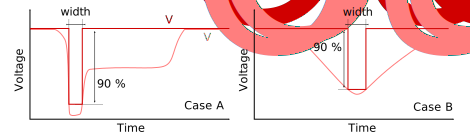
\includegraphics{src/4/figures/better_output_modelling.pdf}
  \caption{Improved output modelling method based on 90\% of maximum disturbance amplitude}
  \label{fig:impact-single-failure-criteria}
\end{figure}

% Result, 2 curves - explain what they are.
